\documentclass{report}
%Needed to use diagbox that make the \ in the table
\usepackage{diagbox}
%Needed to insert any photo
\usepackage{graphicx}
%Needed to insert links
\usepackage{hyperref}

\begin{document}


\chapter*{Ejercicio 4}

Para lograr ver los mintérminos que poseen los bits de salida realizamos la siguinte tabla de verdad:
\begin{center}
	\begin{table}[h!]
		\begin{center}
			\caption{Tabla de Verdad}
			\begin{tabular}{|c|c|}
				\hline
				\textbf{INPUT} & \textbf{OUTPUT} \\
				\hline
				0 0 0 0 & 0 0 0 0\\
				\hline
				0 0 0 1 & 1 1 1 1\\
				\hline
				0 0 1 0 & 1 1 1 0\\
				\hline
				0 0 1 1 & 1 1 0 1\\
				\hline
				0 1 0 0 & 1 1 0 0\\
				\hline
				0 1 0 1 & 1 0 1 1\\
				\hline
				0 1 1 0 & 1 0 1 0\\
				\hline
				0 1 1 1 & 1 0 0 1\\
				\hline
				1 0 0 0 & 1 0 0 0\\
				\hline
				1 0 0 1 & 0 1 1 1\\
				\hline
				1 0 1 0 & 0 1 1 0\\
				\hline
				1 0 1 1 & 0 1 0 1\\
				\hline
				1 1 0 0 & 0 1 0 0\\
				\hline
				1 1 0 1 & 0 0 1 1\\
				\hline
				1 1 1 0 & 0 0 1 0\\
				\hline
				1 1 1 1 & 0 0 0 1\\
				\hline
			\end{tabular} \\
		\end{center}
	\end{table}
\end{center}
Siendo X el primer bit de la izquierda,Y el segundo, W el tercero y Z el ultimo del OUTPUT; y  siendo A el primer bit de la izquierda,B el segundo,C el tercero y D el ultimo. Obtenemos las siguentes salidas dadas en funcion de los minterminos:
	$$ X= m1+m2+m3+m4+m5+m6+m7+m8$$ 
	$$ Y = m1+m2+m3+m4+m9+m10+m11+m12$$
	$$ W = m1+m2+m5+m6+m9+m10+m13+m14$$
	$$ Z = m1+m3+m5+m7+m9+m11+m13+m15$$
Reemplazando los minterminos mi por sus respectivos valores nos queda la siguiente repuesta:
	\begin{center}
		$$ X =  \overline{A} \cdot \overline{B} \cdot \overline{C} \cdot D  +  \overline{A} \cdot \overline{B} \cdot C \cdot \overline{D} + \overline{A} \cdot \overline{B} \cdot C \cdot D + \overline{A} \cdot B \cdot \overline{C} \cdot \overline{D} + \overline{A} \cdot B \cdot \overline{C} \cdot D + \overline{A} \cdot B \cdot C \cdot \overline{D} + \overline{A} \cdot B \cdot C \cdot D+  A \cdot \overline{B} \cdot \overline{C} \cdot \overline{D} $$
$$ Y =  \overline{A} \cdot \overline{B} \cdot \overline{C} \cdot D  +  \overline{A} \cdot \overline{B} \cdot C \cdot \overline{D} + \overline{A} \cdot \overline{B} \cdot C \cdot D + \overline{A} \cdot B \cdot \overline{C} \cdot \overline{D} + A \cdot \overline{B} \cdot \overline{C} \cdot D + A \cdot \overline{B} \cdot C \cdot \overline{D} + A \cdot \overline{B} \cdot C \cdot D+  A \cdot B \cdot \overline{C} \cdot \overline{D} $$
$$ W =  \overline{A} \cdot \overline{B} \cdot \overline{C} \cdot D  +  \overline{A} \cdot \overline{B} \cdot C \cdot \overline{D} + \overline{A} \cdot B \cdot \overline{C} \cdot D + \overline{A} \cdot B \cdot C \cdot \overline{D} + A \cdot \overline{B} \cdot \overline{C} \cdot D + A \cdot \overline{B} \cdot C \cdot \overline{D} + A \cdot B \cdot \overline{C} \cdot D+  A \cdot B \cdot C \cdot \overline{D} $$
$$ Z =  \overline{A} \cdot \overline{B} \cdot \overline{C} \cdot D  +  \overline{A} \cdot \overline{B} \cdot C \cdot D + \overline{A} \cdot B \cdot \overline{C} \cdot D + \overline{A} \cdot B \cdot C \cdot D + A \cdot \overline{B} \cdot \overline{C} \cdot D + A \cdot \overline{B} \cdot C \cdot \overline{D} + A \cdot B \cdot \overline{C} \cdot D+  A \cdot B \cdot C \cdot D $$
	\end{center}
Procedemos a hacer las tablas de Karnaugh de todas las salidas:
\begin{center}
	\begin{table}[h!]
		\begin{center}
			\caption{Tabla de Karnaugh para X}
			\begin{tabular}{|c|c|c|c|c|}
				\hline
				\diagbox{C D} {A B} & \textbf{0 0} & \textbf{0 1} & \textbf{1 1} & \textbf{1 0}  \\
				\hline
				0 0  & 0 & 1 & 0 & 1\\
				\hline
				0 1 & 1 & 1 & 0 & 0 \\
				\hline
				1 1 & 1 & 1 & 0 & 0\\
				\hline
				1 0 & 1 & 1 & 0 & 0\\
				\hline
			\end{tabular} \\
		\end{center}
	\end{table}
\end{center}
\begin{center}
	\begin{table}[h!]
		\begin{center}
			\caption{Tabla de Karnaugh para Y}
			\begin{tabular}{|c|c|c|c|c|}
				\hline
				\diagbox{C D}{A B} & 0 0 & 0 1 & 1 1 & 1 0 \\
				\hline
				0 0  & 0 & 1 & 1 & 0\\
				\hline
				0 1 & 1 & 0 & 0 & 1\\
				\hline
				1 1 & 1 & 0 & 0 & 1\\
				\hline
				1 0 & 1 & 0 & 0 & 1\\
				\hline
			\end{tabular} \\
		\end{center}
	\end{table}
\end{center}
\begin{center}
	\begin{table}[h!]
		\begin{center}
			\caption{Tabla de Karnaugh para W}
			\begin{tabular}{|c|c|c|c|c|}
				\hline
				\diagbox{C D}{A B} & 0 0 & 0 1 & 1 1 & 1 0 \\
				\hline
				0 0  & 0 & 0 & 0 & 0\\
				\hline
				0 1 & 1 & 1 & 1 & 1\\
				\hline
				1 1 & 0 & 0 & 0 & 0\\
				\hline
				1 0 & 1 & 1 & 1 & 1\\
				\hline
			\end{tabular} \\
		\end{center}
	\end{table}
\end{center}
\begin{center}
	\begin{table}[h!]
		\begin{center}
			\caption{Tabla de Karnaugh para Z}
			\begin{tabular}{|c|c|c|c|c|}
				\hline
				\diagbox{C D}{A B} & 0 0 & 0 1 & 1 1 & 1 0 \\
				\hline
				0 0  & 0 & 0 & 0 & 0\\
				\hline
				0 1 & 1 & 1 & 1 & 1\\
				\hline
				1 1 & 1 & 1 & 1 & 1\\
				\hline
				1 0 & 0 & 0 & 0 & 0\\
				\hline
			\end{tabular} \\
		\end{center}
	\end{table}
\end{center}
Luego de seleccionar los grupos correspondientes, las simplificaciones nos quedan:
\begin{center}
		$$ X =  A \cdot \overline{B} \cdot \overline{C} \cdot \overline{D} +\overline{A} \cdot B +\overline{A} \cdot C +\overline{A} \cdot D$$
		$$ Y =  B \cdot \overline{C} \cdot \overline{D}  +  \overline{B} \cdot C + \overline{B} \cdot D $$
		$$ W = \overline{C} \cdot D  + C \cdot \overline{D} $$
		$$ Z =   D $$
\end{center}
De las simplificaciones obtenemos el siguente circuito logico que fue probado y armado en \href{https://logic.ly/demo/}{https://logic.ly/demo/}.
\begin{figure}[h!]
	\centering
	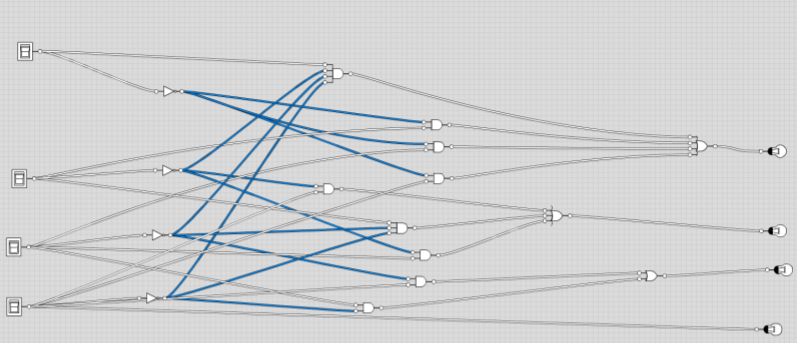
\includegraphics[width=\linewidth]{CircuitoLogico.png}
	\caption{Circuito logico}
\end{figure}

\end{document}